\documentclass{article}
\addtolength{\oddsidemargin}{-1.cm}
\addtolength{\textwidth}{2cm}
\addtolength{\topmargin}{-2cm}
\addtolength{\textheight}{3.5cm}
\newcommand{\HRule}{\rule{\linewidth}{0.5mm}}
\makeindex

\usepackage{longtable}
\usepackage[pdftex]{graphicx}
\usepackage{makeidx}
\usepackage{hyperref}


\usepackage{changepage,lipsum,titlesec}% http://ctan.org/pkg/{changepage,lipsum,titlesec}
\titleformat{\section}[block]{\bfseries}{\thesection.}{1em}{}
\titleformat{\subsection}[block]{}{\thesubsection}{1em}{}
\titleformat{\subsubsection}[block]{}{\thesubsubsection}{1em}{}
\titlespacing*{\subsection} {2em}{3.25ex plus 1ex minus .2ex}{1.5ex plus .2ex}
\titlespacing*{\subsubsection} {3em}{3.25ex plus 1ex minus .2ex}{1.5ex plus .2ex}

\setlength\parindent{74pt}
 
\hypersetup{
	colorlinks=true,
	linkcolor=black,
	filecolor=magenta,      
	urlcolor=cyan,
}


% define the title
\author{Dronr}
\title{ User Manual}

\title{for Now.next}

\begin{document}
	\setlength{\parskip}{6pt}
	
	% generates the title
	\begin{titlepage}
		
		\begin{center}
			% Upper part of the page       
		
			\textsc{\LARGE Dronr}\\[1.5cm]
			\textsc{\Large User Manual}\\[0.5cm]
			% Title
			\HRule \\[0.4cm]
			%%\includegraphics[width=0.05\textwidth]{./retrorabbitLogo}\\[0.4cm] 
			{ \huge \bfseries Group members}\\[0.3cm]
			\HRule \\[0.3cm]
			% Author and supervisor
			\begin{minipage}{0.4\textwidth}
				\begin{flushleft} \large
					\emph{Names:}
				\end{flushleft}
			\end{minipage}
			\begin{minipage}{0.4\textwidth}
				\begin{flushright} \large
					\emph{Student number:}
				\end{flushright}
			\end{minipage}
			
			\begin{minipage}{0.4\textwidth}
				\begin{flushleft} \large
					Vuyani {Shabangu}
				\end{flushleft}
			\end{minipage}
			\begin{minipage}{0.4\textwidth}
				\begin{flushright} \large
					\emph{}
					11171139
				\end{flushright}
			\end{minipage}
			
			\begin{minipage}{0.4\textwidth}
				\begin{flushleft} \large
					Sibusiso {Masemola}
				\end{flushleft}
			\end{minipage}
			\begin{minipage}{0.4\textwidth}
				\begin{flushright} \large
					\emph{}
					12270467
				\end{flushright}
			\end{minipage}
			
			\begin{minipage}{0.4\textwidth}
				\begin{flushleft} \large
					Sello {Thosago}
				\end{flushleft}
			\end{minipage}
			\begin{minipage}{0.4\textwidth}
				\begin{flushright} \large
					\emph{}
					13062060
				\end{flushright}
			\end{minipage}
			
			\begin{minipage}{0.4\textwidth}
				\begin{flushleft} \large
					Banele {Nxumalo}
				\end{flushleft}
			\end{minipage}
			\begin{minipage}{0.4\textwidth}
				\begin{flushright} \large
					\emph{}
					12201911
				\end{flushright}
			\end{minipage}
			
			\begin{minipage}{0.4\textwidth}
				\begin{flushleft} \large
					Aiden {Malan}
				\end{flushleft}
			\end{minipage}
			\begin{minipage}{0.4\textwidth}
				\begin{flushright} \large
					\emph{}
					12265731
				\end{flushright}
			\end{minipage}
			
			
			\vfill
			
		\end{center}
	\end{titlepage}
	\footnotesize
	%\input{declaration_of_originality.tex}
	\normalsize
	
	
	\pagenumbering{roman}
	\tableofcontents
	\newpage
	\pagenumbering{arabic}
	
		\section{Glossary}
		
		\begin{itemsize}  
			
		\item Git - A free and open source distributed version control system de
		signed to handle from small to very large projects with speed
		and efficiency.
		
		\item Git hub - Web-based Git repository hosting service, which allows all of
		the distributed revision control and source code management 
		functionality of Git.
		
		\item Dronr - The System developed to cater on demand drone services at affordable costs.
		
		\end{itemsize}  
		
		\section{Project Repository}
		   https://github.com/vuyaniShabangu/now.next.git
            
		\section{Introduction}
		This is the user manual for dronr – Drone mission control project, with this manual 
		We provide the user with ways on how to use the online portal across any of their desired web browser. 	
	  
	   	{\paragraph}  
	   	This User manual will be providing in depth explanation of the system, starting with setting up on environment to performing operations the systems provides.
	   
\section{Purpose and Overview}		
			
	\subsection{Purpose}
		Dronr was created to explore the growing market of drones as opposed to just being a novelty item, but to be better utilised for various efficient aerial services at lower costs, within less time. Dronr achieves this though providing the consumer a “shopping list” of highly sophisticated drone services such as an orthorectified photo of a given area, with the use of new technology and surveillance algorithms.  
			
			
	\subsection{Overview}
		The dronr is an online service that provides you with the opportunity to use drone services that involve geographical image processing operations, areal inspections, photography, video surveillance and flight operations. This will make it much accessible for you and companies to have such services at a click of a button to the online portal through a browser, and later receive the result of missions you created and submitted to dronr. All missions are to be completed by drone operators then submit results to dronr, which broadcasts them to your portal after being notified that your mission has been completed.
		

					
	\section{General Description}
		\subsection{Browser Client (Users)}
			
			\begin{itemson}
				\item Browser sends requests from user.
				\item Submits mission created 
			\end{itemson}
				
				
			\subsubsection{Server Client (Operator)}
			
			\begin{itemson}
				\item 	Handles the request submitted from browser client, by performing the mission chosen.
				
				\item	Submits the results to the system for any further processing.
			\end{itemson}
			
			\subsection{System}
    	    \begin{itemson}
				\item Uploads the results to the specific client portal.
			\end{itemson}
				
				
			\subsubsection{System configuration}
			 \begin{item}
			 	\item •	Dronr runs on any of your favourite web browser, that support google maps. 
			 \end{item}	
				
	\section{How to use Instructions}%%for normal users and operators.
			
		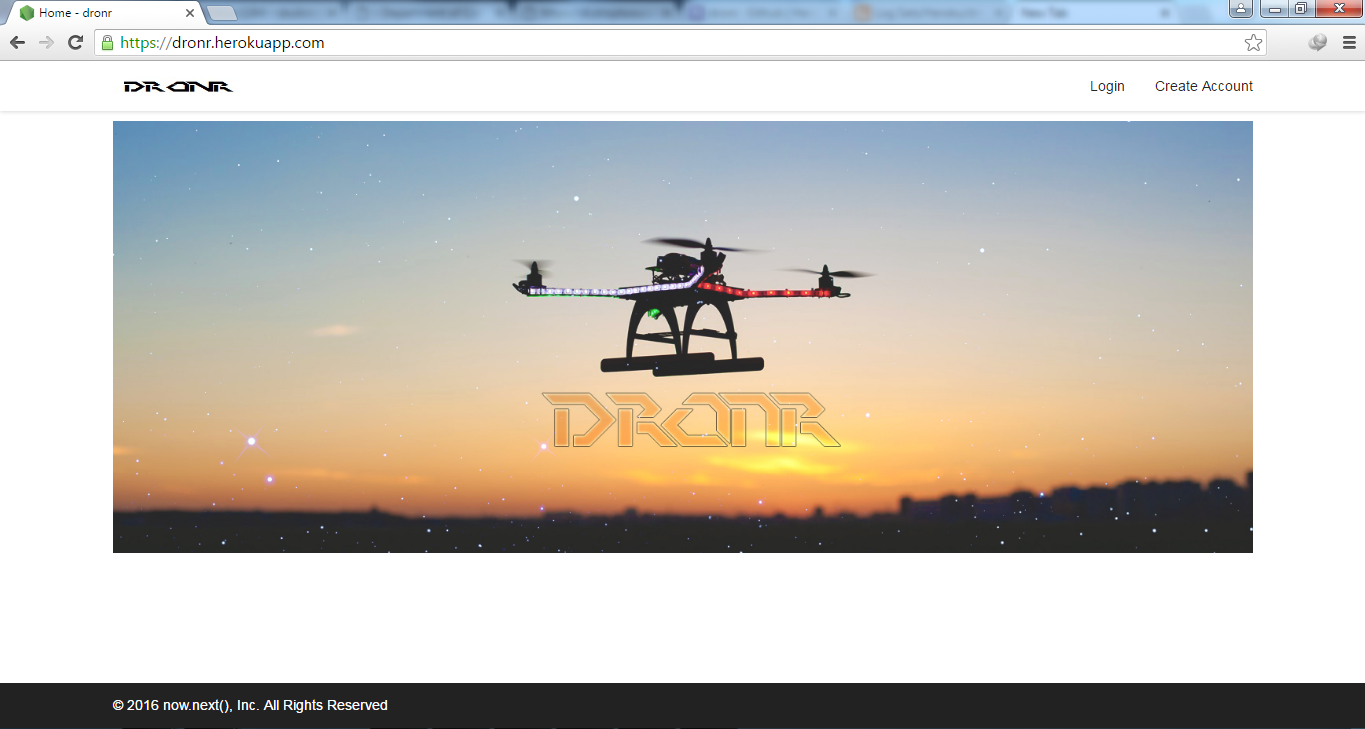
\includegraphics[width=1\textwidth]{./image/homepage.png}\\[0.4cm]
				
		\subsection{Signing Up for Dronr}
		
		
	
		Visit the Dronr website at   https://dronr.herokuapp.com,
		Dronr allows you to create a drone mission and submit it for completion by  independent drone operators listed in the company.
		
		\begin{useritems}
			
			\item {\bfseries on Clicking the Sign Up link.} You will be asked to  create your  portal account. Dronr will ask for your email, password, user name, surname, type of account (operator or normal user), phone number.
			
			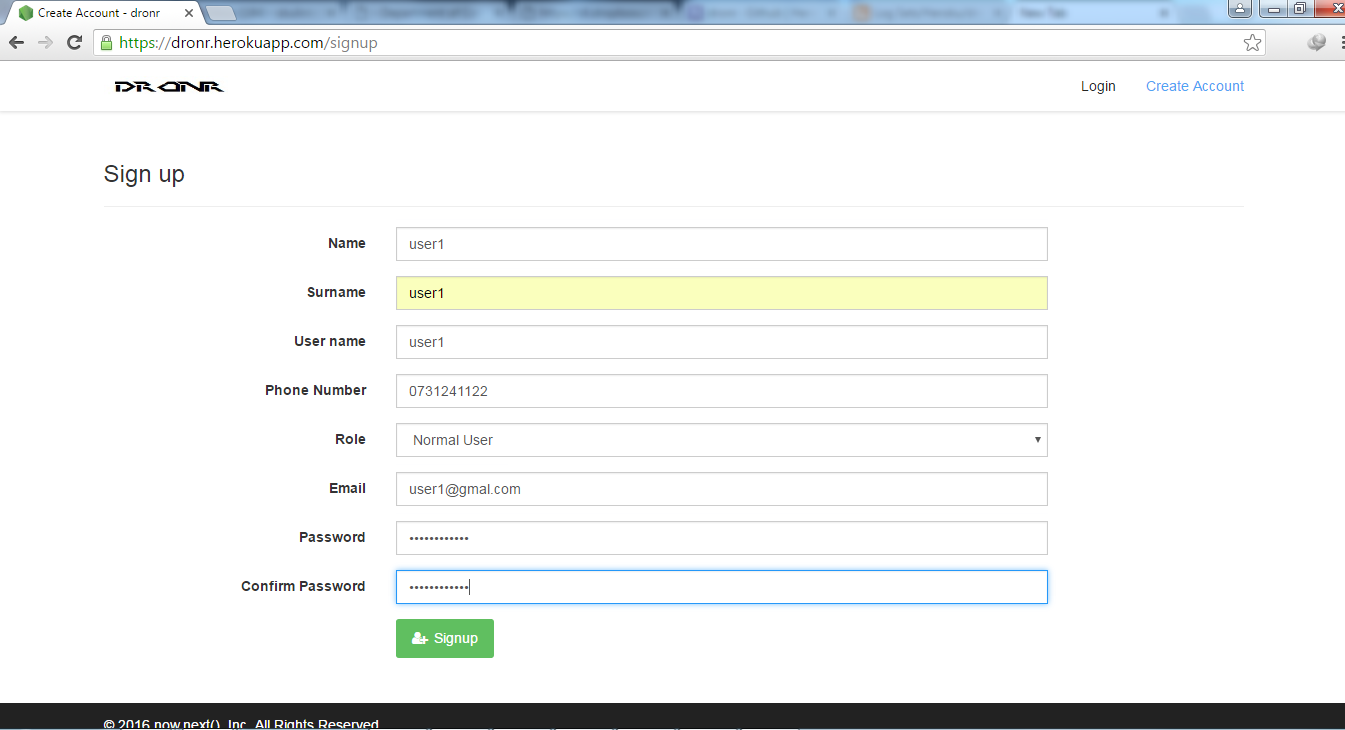
\includegraphics[width=1\textwidth]{./image/SignUp.png}\\[0.4cm]
			
			
			\item read the terms and conditions. Make sure you fully understand the terms and conditions that entail more information about our privacy policy before confirming your sign up, by clicking sign Up link. 
			
			\item {\bfseries Creating a Mission.} The Dronr online service is available on-demand.
			
			\item {\bfseries Sign in.} Once you've successfully registered, You will be logged in automatically, but please keep your password safe for next time when you visit the site and authentication credentials are needed.  
			
			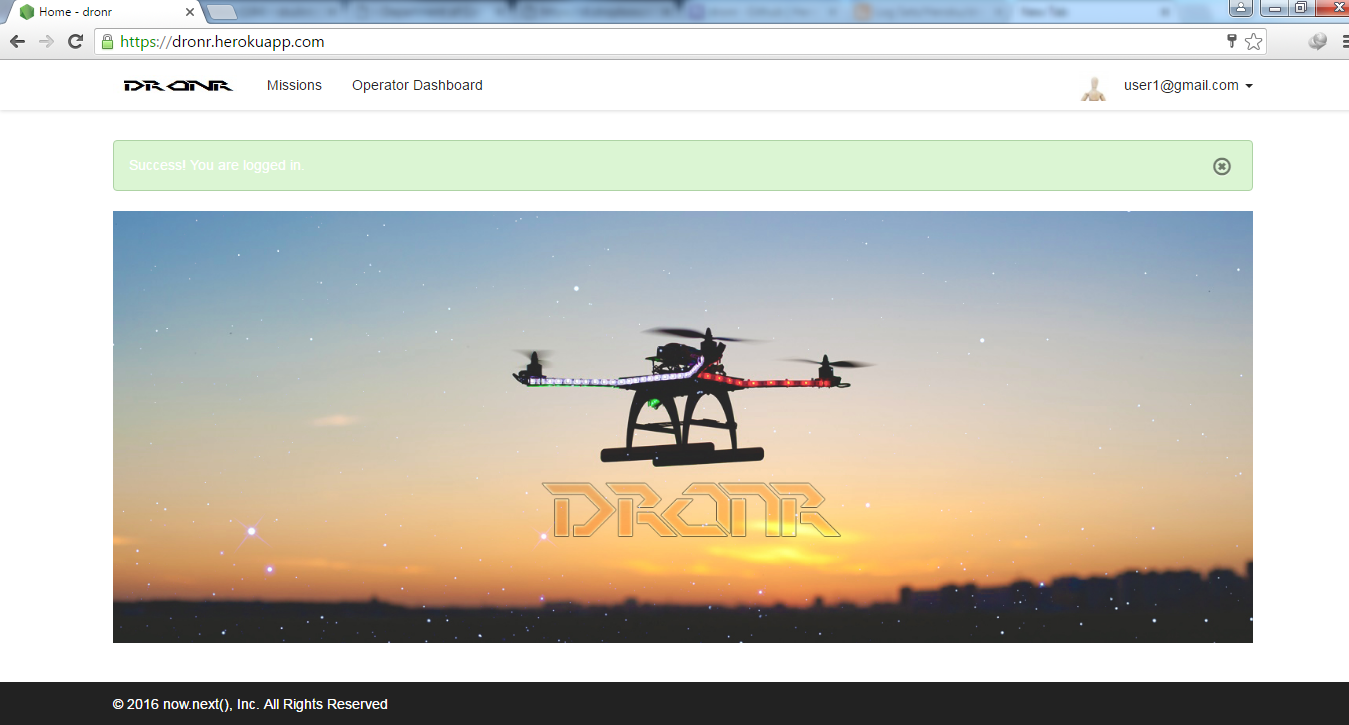
\includegraphics[width=1\textwidth]{./image/LoggedIn.png}\\[0.4cm]			
			
			
			\item {\bfseries Choose Add Mission link.} The missions menu shows all available options for missions, click option 1. 'Add Mission' .
			There are three two types of missions:
			
				
			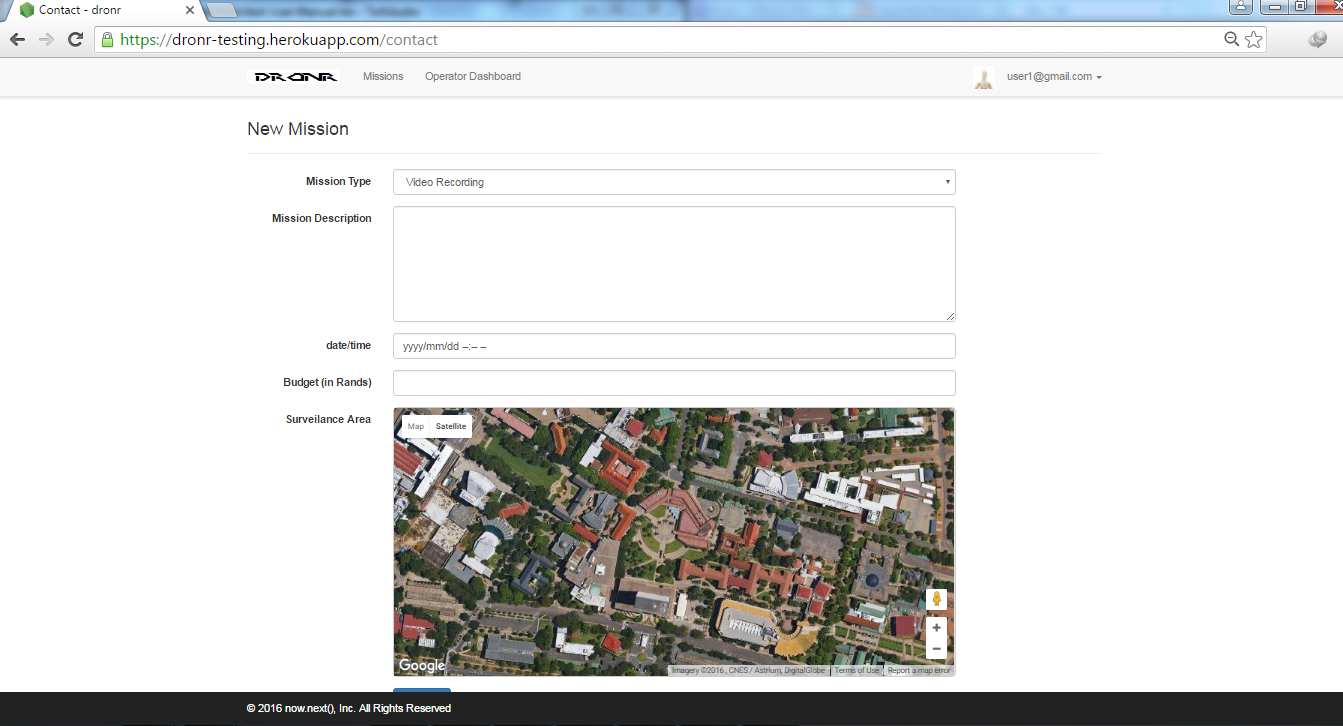
\includegraphics[width=1\textwidth]{./image/AddMission.png}\\[0.4cm]			
			
			\item{Video recording} – Choosing Video recording will be completed depending on compatible drones and video duration; secondly, in mission description text box, please provide a 
			Clear description of what your video should contain; thirdly, in budget text box please provide an estimate of how much you can afford to pay for the mission; in addition, provide the time when your mission is due. Eventually, in map location, please mark your desired mission location on the map provided, select your 1st point, which is a point of take-off, for the drone, next points as well, until return to take-off point; lastly, your way points will allow you to add altitude for the drone to fly at during mission.  
			
			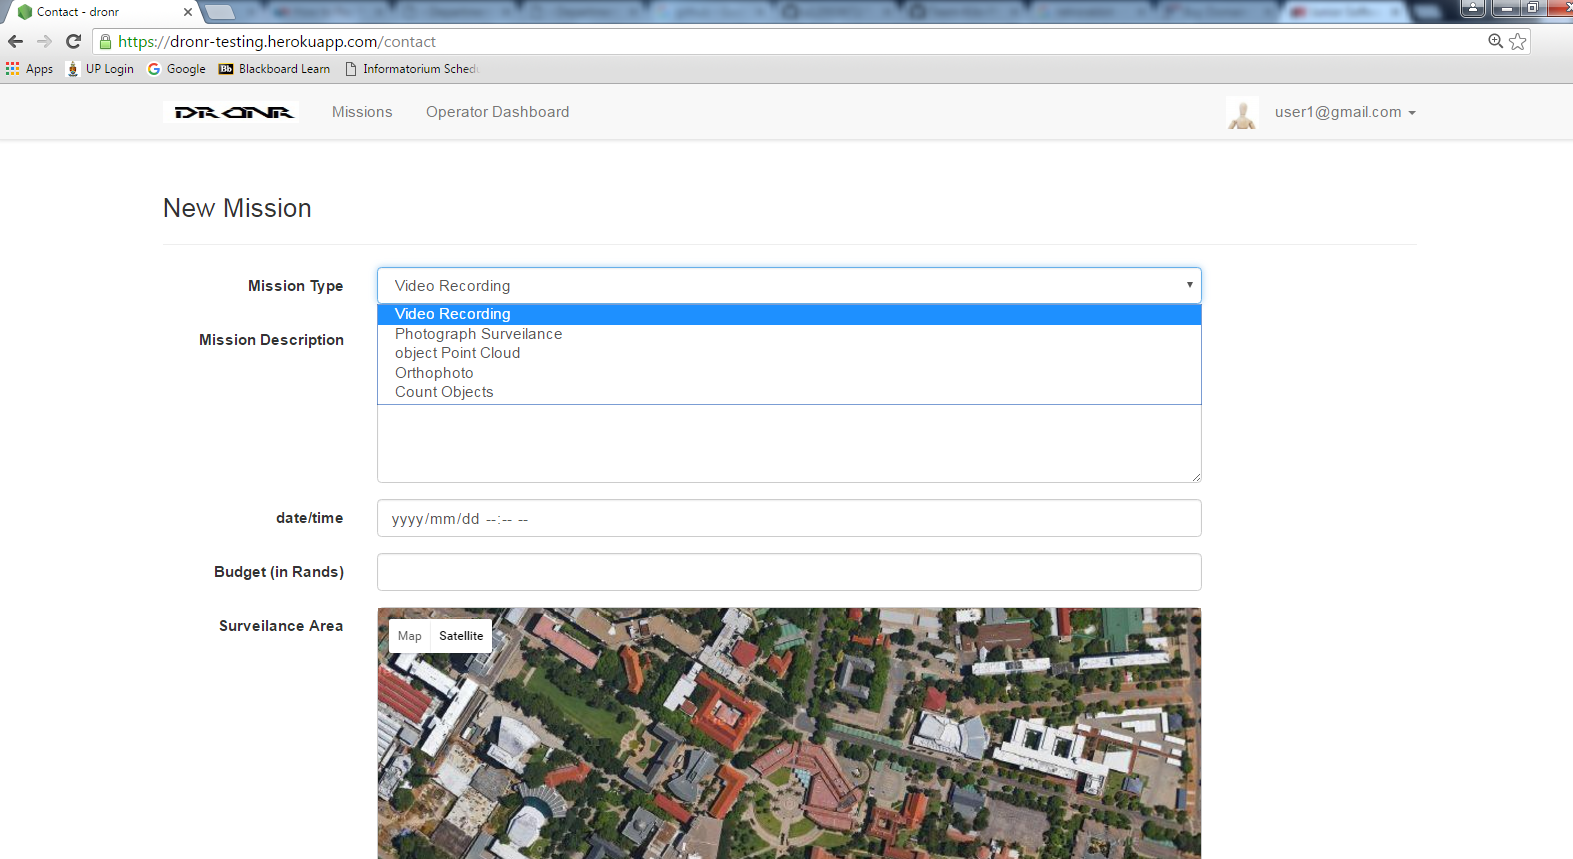
\includegraphics[width=1\textwidth]{./image/missiontypes.png}\\[0.4cm]
				
			\item{Photograph} – Choosing photograph will be completed quicker; secondly, in mission description text box, please provide a 
			Clear description of what your picture should be, a multiple point, single point, cloud point image; thirdly, in budget text box please provide an estimate of how much you can afford to pay for the mission; in addition, provide the time when your mission is due. Eventually, in map location, please mark your desired mission location on the map provided, mark your 1st point, which is a point of take-off, for the drone, next points as well, until return to take-off point; lastly, your way points will allow you to add altitude for the drone to fly at during mission.   
			
			
			\item{\bfseries Mission confirmation. } On completion of filling in mission details, you will be asked to confirm this mission.
			
			
			\item{\bfseries Wait for mission to be accepted.} When your mission is accepted by the drone operator, you will be notified.  Finally your mission will be executed by the qualified operator listed on our system. 
			
			\item{\bfseries View Completed Mission results.}When the drone operator has successfully completed your mission, you will be notified and can find results of your mission on the portal, 1st Click on view my
			missions, select the mission with completed status, you can download or view mission.
		\end{useritems}
		
		
	
\end{document}
